\documentclass[12pt,a4paper]{report}

\usepackage[a4paper,margin=1in]{geometry}
\usepackage{setspace}
\usepackage{graphicx}
\usepackage{amsmath,amssymb,amsfonts}
\usepackage{booktabs}
\usepackage{array}
\usepackage{caption}
\usepackage{float}
\usepackage{titlesec}
\usepackage{enumitem}
\usepackage[hidelinks]{hyperref}
\usepackage{mathtools}
\usepackage{matlab-prettifier}
\usepackage{graphicx} 
\usepackage{caption,subcaption}



\setstretch{1.25}

\titleformat{\chapter}[display]
{\normalfont\bfseries\Large}
{\chaptertitlename\ \thechapter}{12pt}{\Large}

\begin{document}
	
	\begin{titlepage}
		\centering
		
		{\Large \textsc{CU Boulder / Coursera} \par}
		\vspace{2cm}
		
		{\Huge \textbf{Spacecraft Dynamics Capstone Project} \par}
		\vspace{1cm}
		
		{\LARGE Attitude Dynamics and Control of a Nano-Satellite Orbiting Mars \par}
		\vspace{2cm}
		
		{\Large Course Report \par}
		\vfill
		
		\begin{flushleft}
			\large
			\textbf{Student:} Haniyeh Zahra Budaqi \\
			\textbf{Instructor:} Prof. Dr. Hanspeter Schaub
		\end{flushleft}
		
		\vspace{2cm}
		
		{\large May 2026 \par}
		
	\end{titlepage}
	
	\tableofcontents
	\newpage
	
	\chapter*{Abstract}
	\addcontentsline{toc}{chapter}{Abstract}
	
	In this project, the knowledge acquired from the Spacecraft Dynamics and Control specialization is applied to perform attitude control of a nano-satellite orbiting Mars while operating as a daughter-craft to a mother spacecraft in a geostationary Mars orbit (GMO). Through the completion and analysis of eleven project tasks, an attitude control architecture is developed and validated. The resulting simulation enables three operational modes based on the spacecraft mission requirements and relative orbital geometry:
	
	\begin{enumerate}[label=\arabic*)]
		\item Science mode: pointing the spacecraft sensor toward the Martian surface,
		\item Power mode: orienting the solar panels toward the Sun,
		\item Communication mode: pointing the communication antenna toward the mother spacecraft.
	\end{enumerate}
	
	The spacecraft dynamics, reference-frame generation, attitude error evaluation, and closed-loop control simulations are implemented in MATLAB, while mission visualization is performed using AGI Systems Tool Kit (STK).
	
	\chapter{Introduction}
	
	This project considers a small science satellite orbiting Mars in a Low Mars Orbit (LMO), tasked with collecting scientific data from the Martian surface and relaying the acquired information to a larger mother spacecraft orbiting in a Geostationary Mars Orbit (GMO). In addition to science and communication operations, the spacecraft must periodically orient its solar panels toward the Sun to maintain sufficient onboard power.
	
	Accordingly, the spacecraft mission is divided into three operational modes:
	
	\begin{enumerate}[label=\arabic*)]
		\item \textbf{Science Mode:} pointing the sensor toward the Martian surface,
		\item \textbf{Power Mode:} orienting the solar panels toward the Sun,
		\item \textbf{Communication Mode:} pointing the communication antenna toward the GMO spacecraft.
	\end{enumerate}
	
	Both the LMO and GMO spacecraft are assumed to follow known circular orbits whose orientations are described using Hill reference frames generated through a 3-1-3 Euler-angle sequence.
	
	The LMO spacecraft is equipped with:
	
	\begin{itemize}
		\item A science sensor aligned with the $+b_1$ body axis,
		\item Solar panels whose normal vector aligns with the $b_3$ axis,
		\item A communication antenna aligned with the $-b_1$ axis.
	\end{itemize}
	
	The objective of this project is to design and validate an attitude determination and control framework capable of autonomously switching between the required operational pointing modes.
	
	\chapter{Mission Scenario Definitions}
	
	\section{Mission Orbit Overview}
	
	The LMO and GMO spacecraft are both assumed to follow circular orbits around Mars. The orbital motion is modeled using classical two-body dynamics, where Mars is treated as the central gravitational body.
	
	The physical and orbital parameters used throughout the simulations are summarized in Table~\ref{tab:simparams}.
	\begin{table}[H]
		\centering
		\caption{Simulation and Spacecraft Parameters}
		\label{tab:simparams}
		\begin{tabular}{lll}
			\toprule
			Parameter & Value & Unit \\
			\midrule
			Mars radius $R_{Mars}$ & 3396.19 & km \\
			Mars gravitational parameter $\mu_{Mars}$ & $4.28283\times10^{13}$ & m$^3$/s$^2$ \\
			LMO altitude & 400 & km \\
			LMO orbital radius $r_{LMO}$ & 3796.19 & km \\
			GMO orbital radius $r_{GMO}$ & 20424.2 & km \\
			LMO orbital angular rate $\dot{\theta}_{LMO}$ & 0.000884797 & rad/s \\
			GMO orbital angular rate $\dot{\theta}_{GMO}$ & 0.0000709003 & rad/s \\
			\bottomrule
		\end{tabular}
	\end{table}
	
	The orbital angular rates are computed using the circular-orbit relation:
	
	\[
	\dot{\theta} = \sqrt{\frac{\mu_{Mars}}{r^3}}
	\]
	
	The initial orbit orientation angles of both spacecraft are summarized in Table~\ref{tab:orbitangles}.
	
	\begin{table}[H]
		\centering
		\caption{Initial Orbit Frame Orientation Angles}
		\label{tab:orbitangles}
		\begin{tabular}{cccc}
			\toprule
			Spacecraft & $\Omega$ (deg) & $i$ (deg) & $\theta(t_0)$ (deg) \\
			\midrule
			LMO & 20 & 30 & 60 \\
			GMO & 0 & 0 & 250 \\
			\bottomrule
		\end{tabular}
	\end{table}
	Figure~\ref{fig:orbits_frames} illustrates the definition of a circular orbit using relative elements along with inertial and Hill frames' base vectors. Note that the orbital elements ($\Omega,i,\theta$) can be used as (3-1-3) Euler Angles to obtain Hill frame $\mathcal{H}$ from inertial frame $\mathcal{N}$.
	
	\begin{figure}[H]
		\centering
		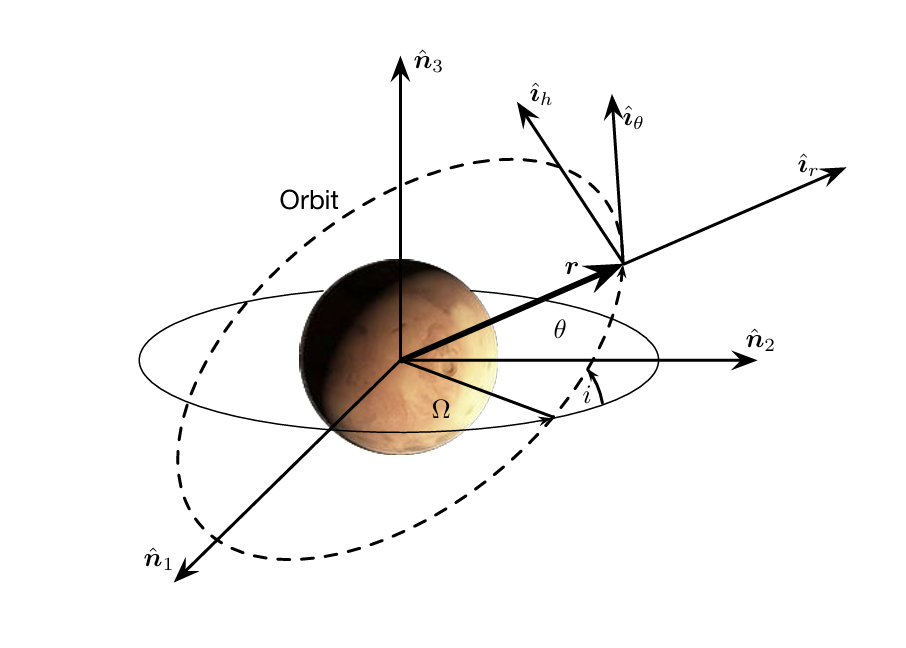
\includegraphics[width=0.7\textwidth]{figures/doc_orbits_frames.png}
		\caption{Illustration of circular orbital elements alongside inertial frame $\mathcal{N} : \{\boldsymbol{\hat{n}}_1, \boldsymbol{\hat{n}}_2, \boldsymbol{\hat{n}}_3\}$ and Hill frame $\mathcal{H} : \{\boldsymbol{\hat{i}}_r, \boldsymbol{\hat{i}}_\theta, \boldsymbol{\hat{i}}_h\}$ base vectors}
		\label{fig:orbits_frames}
	\end{figure}
	
	\section{Mission Pointing Scenarios}
	
	A body frame as shown in Figure~\ref{fig:lmo_body_frame} is mounted on the spacecraft, assuming to be the principle body frame. 
	
	\begin{figure}[H]
		\centering
		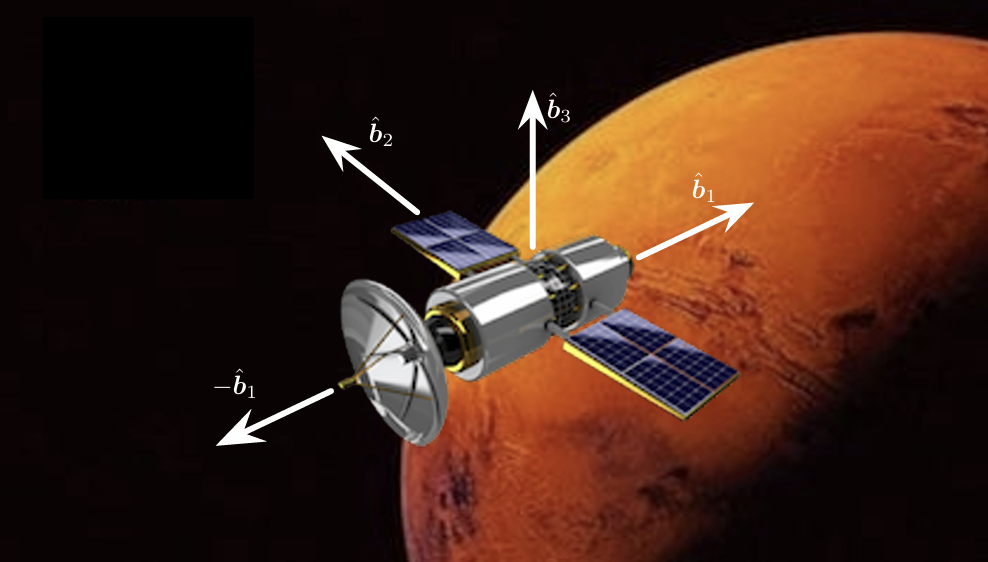
\includegraphics[width=0.7\textwidth]{figures/lmo_body_frame.png}
		\caption{Illustration of LMO spacecraft's body frame $\mathcal{B}:\{\boldsymbol{\hat{b}}_1, \boldsymbol{\hat{b}}_2, \boldsymbol{\hat{b}}_3\}$}
		\label{fig:lmo_body_frame}
	\end{figure}
	
	Three operational spacecraft pointing modes are defined according to mission requirements.
	
	The Sun is assumed to be located at an effectively infinite distance and aligned with the inertial $n_2$ axis. Therefore, during Sun-pointing operation, the spacecraft solar-panel axis $b_3$ must align with the inertial $n_2$ direction.
	
	The spacecraft operational modes are summarized as follows:
	
	\begin{itemize}
		\item \textbf{Power Mode:} active whenever the spacecraft is on the sunlit side of Mars,
		\item \textbf{Science Mode:} active during eclipse when GMO communication is unavailable,
		\item \textbf{Communication Mode:} active whenever the GMO spacecraft lies within the communication visibility constraint.
	\end{itemize}
	
	The communication mode is activated when the angular separation between the LMO and GMO position vectors is less than $35^{\circ}$.
	
	\begin{table}[H]
		\centering
		\caption{Mission Pointing Scenario Summary}
		\label{tab:pointing}
		\begin{tabular}{ll}
			\toprule
			Orbital Situation & Operational Mode\\
			\midrule
			Spacecraft on sunlit Mars side & Power Mode\\
			Spacecraft in eclipse and GMO visible & Communication Mode \\
			Spacecraft in eclipse and GMO not visible & Science Mode\\
			\bottomrule
		\end{tabular}
	\end{table}
	
	\begin{figure}[H]
		\centering
		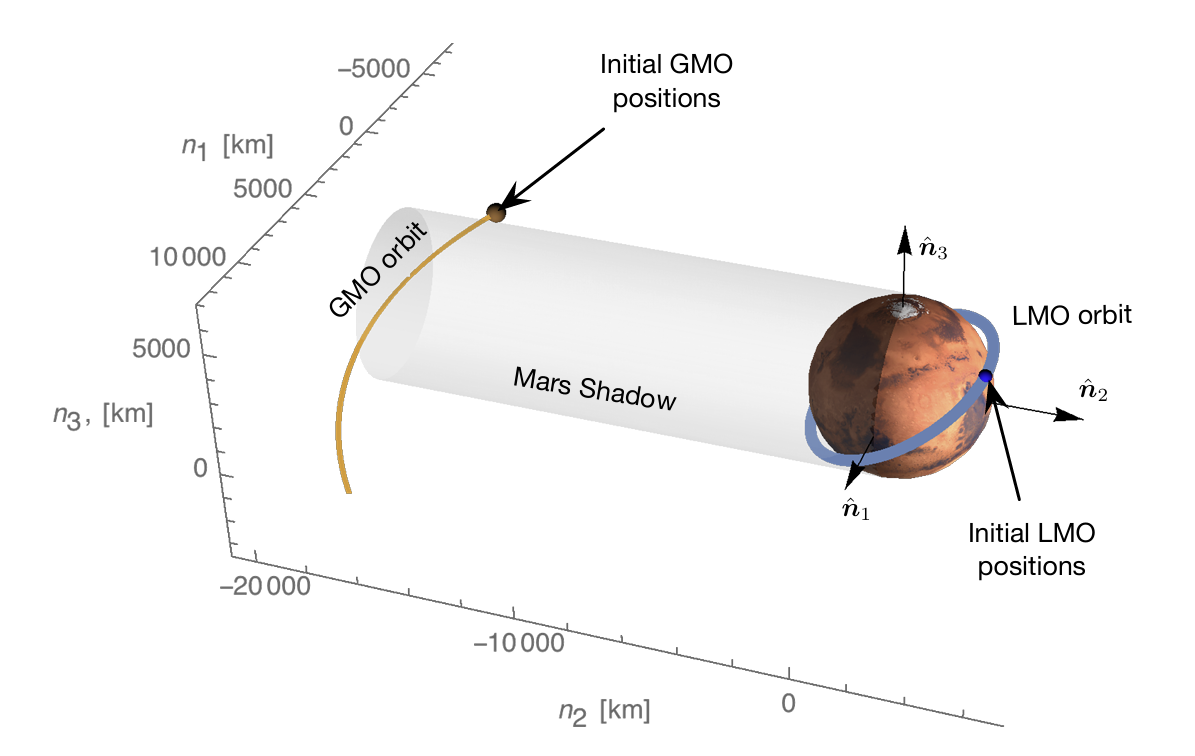
\includegraphics[width=1.0\textwidth]{figures/orbit_scenario.png}
		\caption{Mission Orbit Scenario Illustration}
		\label{fig:orbit_scenario}
	\end{figure}
	
	\section{Spacecraft Attitude States}
	
	The spacecraft initial attitude is represented using Modified Rodrigues Parameters (MRPs), while the initial angular velocity is expressed in the spacecraft body frame.
	
	The initial spacecraft attitude is defined as:
	
	\[
	\boldsymbol{\sigma}_{B/N}(t_0) =
	\begin{bmatrix}
		0.3 \\
		-0.4 \\
		0.5
	\end{bmatrix}
	\]
	
	The initial body angular velocity is:
	
	\[
	{\prescript{\mathcal{B}}{}{\boldsymbol{\omega}}}_{B/N}(t_0) =
	\begin{bmatrix}
		1.00 \\
		1.75 \\
		-2.20
	\end{bmatrix}
	deg/s
	\]
	
	The rigid-body spacecraft inertia tensor is assumed to be:
	
	\[
	\prescript{\mathcal{B}}{}{[I]} =
	\prescript{\mathcal{B}}{}{\begin{bmatrix}
			10 & 0 & 0 \\
			0 & 5 & 0 \\
			0 & 0 & 7.5
	\end{bmatrix}}
	\text{ kg·m}^2
	\]
	
	The spacecraft is assumed to be capable of generating arbitrary three-axis control torques through an onboard actuator system.
	
	\section{Attitude Control Law Overview}
	
	A proportional-derivative (PD) control law is used throughout this project to regulate spacecraft attitude motion:
	
	\[
	\prescript{\mathcal{B}}{}{\mathbf{u}} = -K\boldsymbol{\sigma}_{B/R} - P\prescript{\mathcal{B}}{}{\boldsymbol{\omega}}_{B/R}
	\]
	
	where:
	
	\begin{itemize}
		\item $\boldsymbol{\sigma}_{B/R}$ is the attitude tracking error,
		\item $\prescript{\mathcal{B}}{}{\boldsymbol{\omega}}_{B/R}$ is the angular velocity tracking error,
		\item $K$ and $P$ are controller gain matrices.
	\end{itemize}
	
	The objective of the controller is to detumble the spacecraft while driving the body frame toward a desired mission reference frame.
	 
	\section{Implementation Methods}
	
	[NEED REVISION BEFORE EVEN BEING WRITTEN]
	
	\chapter{Task Descriptions and Solutions}
	
	\section{Orbits}
	
	\subsection{Task 1: Orbit Simulation}
	
	Assume the general orbit frame as $\mathcal{O}: \{\hat{i}_r, \hat{i}_\theta, \hat{i}_h\}$. Even though the general orbit frame and Hill frame basically use the same base vectors, their difference is found in their origin. $\mathcal{O}$ frame has its origin aligned with the origin of inertial frame $\mathcal{N}$ -- which is the center of Mars. The Hill frame $\mathcal{H}$, however, is mounted on the spacecraft, therefore has the same origin as the body frame $\mathcal{B}$. 
	
	Both these frames are obtainable through a (3-1-3) Euler Angle rotation on the inertial frame, though the hill frame origin is also translated to the spacecraft. 
	
	Now, using the $\mathcal{O}$ frame, spacecraft position vector is expressed as:
	$$\prescript{\mathcal{O}}{}{\boldsymbol{r}} = r\boldsymbol{\hat{i}}_r$$
	
	Both LMO and GMO orbits are circular, therefore having the same angular velocity $\dot{\theta}$ all over the orbit. Spacecraft velocity vector is expressed as:
	$$\prescript{\mathcal{O}}{}{\boldsymbol{\dot{r}}} = r\dot{\theta}\boldsymbol{\hat{i}}_\theta$$
	
	The MATLAB function \texttt{orbitTheta()} takes time, angular velocity and initial angle to calculate the element $\theta$ using the following equation:
	$$\theta_t = \dot{\theta}t + \theta_0$$
		
	Taking the position and velocity vectors from the general orbit frame to the inertial frame is done using the DCM $[NO]$ which can be obtained having all orbital elements at a given time.
	$$[ON] = M_3(\theta_t)M_1(i)M_3(\Omega)$$
	$$[NO] = [ON]^T$$
	$$\prescript{\mathcal{N}}{}{\boldsymbol{r}} = [NO] \prescript{\mathcal{O}}{}{\boldsymbol{r}}$$
	$$\prescript{\mathcal{N}}{}{\boldsymbol{\dot{r}}} = [NO] \prescript{\mathcal{O}}{}{\boldsymbol{\dot{r}}}$$
	
	This is achieved by the MATLAB function \texttt{orbit\_state()}.
	
	
	\subsection{Task 2: Orbit Frame Orientation}
	
	The Hill-frame basis vectors were constructed directly from the inertial position and velocity vectors:
	
	\[
	\prescript{\mathcal{N}}{}{\boldsymbol{\hat{i}}_r} = \frac{\boldsymbol{r}_{LMO}}{\|\boldsymbol{r}_{LMO}\|}
	\]
	
	\[
	\prescript{\mathcal{N}}{}{\boldsymbol{\hat{i}}_h} = \frac{\boldsymbol{r}_{LMO} \times \boldsymbol{\dot{r}}_{LMO}}{\|\boldsymbol{r}_{LMO} \times \boldsymbol{\dot{r}}_{LMO}\|}
	\]
	
	\[
	\prescript{\mathcal{N}}{}{\boldsymbol{\hat{i}}_\theta} = \boldsymbol{\hat{i}}_h \times \boldsymbol{\hat{i}}_r
	\]
	
	To drive a DCM with the base vectors in either frames, we have:
	$$[FB] = 
	\begin{bmatrix}
		\prescript{\mathcal{F}}{}{\hat{\boldsymbol{b}}_1} & \prescript{\mathcal{F}}{}{\hat{\boldsymbol{b}}_2} & \prescript{\mathcal{F}}{}{\hat{\boldsymbol{b}}_3}
	\end{bmatrix} =
	\begin{bmatrix}
		\prescript{\mathcal{B}}{}{\hat{\boldsymbol{f}}_1 ^ T} \\
		\prescript{\mathcal{B}}{}{\hat{\boldsymbol{f}}_2 ^ T} \\
		\prescript{\mathcal{B}}{}{\hat{\boldsymbol{f}}_3 ^ T}
	\end{bmatrix}	$$
	
	Therefore, to find $[HN]$ we will have:
	$$[HN] = 
	\begin{bmatrix}
		\prescript{\mathcal{N}}{}{\boldsymbol{\hat{i}}_r ^ T} \\
		\prescript{\mathcal{N}}{}{\boldsymbol{\hat{i}}_\theta ^ T} \\
		\prescript{\mathcal{N}}{}{\boldsymbol{\hat{i}}_h ^ T}
	\end{bmatrix}$$
	
	A MATLAB function named \texttt{orbit\_frame\_dcm(t)} was implemented to evaluate the time-varying Hill-frame orientation.

	\section{Reference Frame Orientation}
	
	\subsection{Task 3: Sun-Pointing Reference Frame Orientation}
	
	To point the spacecraft solar panels axis $\boldsymbol{\hat{b}}_3$ at the Sun, the reference frame $\mathcal{R}_s$ must be chosen such that $\boldsymbol{\hat{r}}_3$ axis points in the Sun direction ($\boldsymbol{\hat{n}}_2$ in the scenario). To define the frame completely, the first axis $\boldsymbol{\hat{r}}_1$ is assumed to point in $-\boldsymbol{\hat{n}}_1$ direction. Therefore, the base vectors will be:
	
	$$ \boldsymbol{\hat{r}}_1 = -\boldsymbol{\hat{n}}_1 $$
	$$ \boldsymbol{\hat{r}}_3 = \boldsymbol{\hat{n}}_2 $$
	$$ \boldsymbol{\hat{r}}_2 = \boldsymbol{\hat{r}}_3 \times \boldsymbol{\hat{r}}_1 = -(\boldsymbol{\hat{n}}_2\times\boldsymbol{\hat{n}}_1) = \boldsymbol{\hat{n}}_3$$
	
	Similar to the previous task, the analytical expression for the DCM can be obtained using the base vectors:
	
	$$[R_sN] = 
	\begin{bmatrix}
		\prescript{\mathcal{N}}{}{\boldsymbol{\hat{r}}_1 ^ T} \\
		\prescript{\mathcal{N}}{}{\boldsymbol{\hat{r}}_2 ^ T} \\
		\prescript{\mathcal{N}}{}{\boldsymbol{\hat{r}}_3 ^ T}
	\end{bmatrix}
	= \begin{bmatrix}
		-1 & 0 & 0 \\
		0 & 0 & 1 \\
		0 & 1 & 0
	\end{bmatrix}$$
	
	The resulting reference-frame DCM  can also be obtained using a (3-1-3) Euler Angle of ($\pi$, $\frac{\pi}{2}$, 0) rotation on it. MATLAB function $\texttt{RsN\_DCM()}$ serves this purpose.
	
	Since the base vectors of this frame are just a re-arrangement of the inertial frame base vectors, the frame remains fixed relative to the inertial frame, thus:
	
	$$ \boldsymbol{\omega}_{R_s/N} = 0$$

	
	\subsection{Task 4: Nadir-Pointing Reference Frame Orientation}
	
	To point the spacecraft sensor platform axis $ \boldsymbol{\hat{b}}_1 $ towards the center of Mars (nadir direction), the reference frame $\mathcal{R}_n$ must be chosen such that $ \boldsymbol{\hat{r}}_1 $ axis points towards the planet. To completely describe the frame, we assume the second axis $ \boldsymbol{\hat{r}}_2 $ points in velocity direction $ \boldsymbol{\hat{i}}_\theta $. Therefore, we'll have:
	
	$$  \boldsymbol{\hat{r}}_1 = -\boldsymbol{\hat{i}}_r $$
	$$
	 \boldsymbol{\hat{r}}_2 = \boldsymbol{\hat{i}}_\theta 
	$$
	$$ \boldsymbol{\hat{r}}_3 = \boldsymbol{\hat{r}}_1 \times \boldsymbol{\hat{r}}_3 = -\boldsymbol{\hat{i}}_h$$
	
	This frame can be obtained using a (3-1-3) Euler Angles rotation on the Hill frame with angles ($\pi, \pi, 0$).
	
	$$[R_nH] = M_1(\pi)M_3(\pi)$$
	
	
	 We also had previously obtained $[HN]$ in task 2 as a function of time. So,
	 
	 $$[R_nN] (t) = [R_nH][HN](t) $$
	 
	 In MATLAB, this task is done by function \texttt{RnN\_DCM()}.
	
	Since this frame is a re-arrangement of the Hill frame, it also moves with it, thus:
	$$\boldsymbol{\omega}_{R_n/N} = \boldsymbol{\omega}_{H/N} = \dot{\theta}\boldsymbol{\hat{i}}_\theta$$
	 
	
	
	
	\subsection{Task 5: GMO-Pointing Reference Frame Orientation}
	
	To point the nano-satellite communication platform axis $\boldsymbol{\hat{b}}_1$ towards the GMO mother spacecraft, the communication reference frame $\mathcal{R}_c$ must be chosen such that $-\boldsymbol{\hat{r}}_1$ axis points towards the GMO satellite location, defining $\Delta\boldsymbol{r} = \boldsymbol{r}_{GMO} - \boldsymbol{r}_{LMO}$. So,
	$$\boldsymbol{\hat{r}}_1 = -\frac{\Delta\boldsymbol{r}}{\|\Delta\boldsymbol{r}\|}$$
	Further, to fully define a three-dimensional reference frame, assume the second axis is defined as
	$$\boldsymbol{\hat{r}}_2 = \frac{\Delta\boldsymbol{r}\times\boldsymbol{\hat{n}}_3}{\|\Delta\boldsymbol{r}\times\boldsymbol{\hat{n}}_3\|}$$
	Naturally,
	$$\boldsymbol{\hat{r}}_3 = \boldsymbol{\hat{r}}_1 \times \boldsymbol{\hat{r}}_2$$
	
	Having all three base vectors in the inertial frame, we have:
	$$[R_cN] = 
	\begin{bmatrix}
		\prescript{\mathcal{N}}{}{\boldsymbol{\hat{r}}_1 ^ T} \\
		\prescript{\mathcal{N}}{}{\boldsymbol{\hat{r}}_2 ^ T} \\
		\prescript{\mathcal{N}}{}{\boldsymbol{\hat{r}}_3 ^ T} \\
	\end{bmatrix}$$
	
	The MATLAB function \texttt{RcN\_DCM(t)} is written to deliver this task.
	
	To derive the relative angular velocity $\prescript{\mathcal{N}}{}{\boldsymbol{\omega}_{R_c/N}}$, we'll use an equation (3.27) in book $\colorbox{yellow}{give reference later}$ :
	$$[\dot{C}] = -[\tilde{\boldsymbol{\omega}}][C]$$
	Therefore,
	$$[\tilde{\boldsymbol{\omega}}_{R_c/N}] = 
	\begin{bmatrix}
		0 & -\omega_3 & \omega_2 \\
		\omega_3 & 0 & -\omega_1 \\
		-\omega_2 & \omega_1 & 0
	\end{bmatrix} = -[\dot{R_cN}][R_cN]^T$$
	
	To derive the rate of a DCM numerically, we'll have:
	$$[\dot{R_cN}] \approx \frac{[R_cN]_{t+dt} - [R_cN]_{t}}{dt}$$
	
	This algorithm is implemented in MATLAB function \texttt{RcN\_omega(t)}. The choice of different \texttt{dt} will result in different precisions in finding the angular velocity.	
	
	\section{Attitude Evaluation and Simulator}
	
	\subsection{Task 6: Attitude Error Evaluation}
	
	Any attitude feedback control algorithm requires the ability to compute the attitude and angular velocity tracking errors of the current body frame $\mathcal{B}$ relative to the reference frame $\mathcal{R}$. 
	To find a set of tracking errors $\begin{bmatrix}
		\boldsymbol{\sigma}_{B/R} \\
		\prescript{\mathcal{B}}{}{\boldsymbol{\omega}}_{B/R}
	\end{bmatrix}$, we have the known variables $\boldsymbol{\sigma}_{B/N}$, $\prescript{\mathcal{B}}{}{\boldsymbol{\omega}}_{B/N}$, as well as the desired reference frame DCM $[RN]$ and frame rate $\prescript{\mathcal{N}}{}{\boldsymbol{\omega}}_{R/N}$.
	We first need to drive the DCM $[BN]$ which can be obtained from $\boldsymbol{\sigma}_{B/N}$ using equation (3.152):
	$$[C] = [I_{3\times3}] + \frac{8[\tilde{\boldsymbol{\sigma}}]^2 - 4(1-\sigma^2)[\tilde{\boldsymbol{\sigma}}]}{(1+\sigma^2)^2}$$
	
	The opposite of this operation--converting a DCM to its MRP form--is formulated in equation (3.153):
	$$[\tilde{\boldsymbol{\sigma}}] = \frac{[C]^T - [C]}{\zeta(\zeta+2)}$$
	$$\zeta = \sqrt{trace([C])+1}$$ 
	
	These two forms are implemented in MATLAB function \texttt{sigmaToDCM()} and \texttt{DCMToSigma()} in respect. 
	
	Now, the roadmap to finding the tracking errors would be:
	$$\boldsymbol{\sigma}_{B/N} \rightarrow [BN] $$	
	$$[BR] = [BN][NR] = [BN][RN]^T$$
	$$[BR] \rightarrow \boldsymbol{\sigma}_{B/R}$$
	$$\prescript{\mathcal{B}}{}{\boldsymbol{\omega}}_{B/R} = \prescript{\mathcal{B}}{}{\boldsymbol{\omega}}_{B/N} - \prescript{\mathcal{B}}{}{\boldsymbol{\omega}}_{R/N} = \prescript{\mathcal{B}}{}{\boldsymbol{\omega}}_{B/N} - [BN]\prescript{\mathcal{N}}{}{\boldsymbol{\omega}}_{R/N}$$
	
	A MATLAB function named \texttt{attitudeErrorEval()} was implemented to evaluate both attitude and angular velocity tracking errors.
	
	\subsection{Task 7: Numerical Attitude Simulator}
	
	In order to integrate the attitude we need a numerical integrator. The LMO and GMO orbit satellite positions are already calculated in earlier tasks. Let the propagated attitude state $\boldsymbol{X}$ be
	$$\boldsymbol{X} = \begin{bmatrix}
		\boldsymbol{\sigma}_{B/N} \\
		\prescript{\mathcal{B}}{}{\boldsymbol{\omega}}_{B/N}
	\end{bmatrix}$$
	
	Assuming that the spacecraft is rigid and there's no external torque acting on it, its dynamics obey
		
	\[
	[I]\dot{\boldsymbol{\omega}}_{B/N} = - [\tilde{\boldsymbol{\omega}}_{B/N}][I]\boldsymbol{\omega}_{B/N} + \boldsymbol{u} 
	\]
	where $\boldsymbol{u}$ is the external control torque vector.
	
	For this task, a simple loop integrator was written in MATLAB (which comparing to RK4, proved to be more time-consuming yet more precise). The control torques $\boldsymbol{u}_1 = 0$ and $\prescript{\mathcal{B}}{}{\boldsymbol{u}} = (0.01, -0.01, 0.02)$
	were applied respectively and the following were computed:
	\begin{itemize}
		\item Attitude MRP $\boldsymbol{\sigma}_{B/N}$
		\item Angular velocity $\boldsymbol{\omega}_{B/N}$
		\item Angular momentum vector $\boldsymbol{H} = [I]\boldsymbol{\omega}_{B/N}$ in both $\mathcal{N}$ and $\mathcal{B}$ frames
		\item Rotational kinetic energy $T = \frac{1}{2}\boldsymbol{\omega}_{B/N}^T[I]\boldsymbol{\omega}_{B/N}$
	\end{itemize}
	
	The results of both simulations are plotted in Figure~\ref{fig:task7_results}. As is seen, after applying the control torque $\boldsymbol{u}_2$ on the spacecraft, its rotational kinetic energy plummets (from approximately 9 mJ in uncontrolled mode (Figure~\ref{fig:u1_T}) to more than 2.5 J when controlled (Figure~\ref{fig:u2_T})). This is verified by spacecraft angular velocity, whose 1st and 2nd components start to oscillate in controlled mode while its 3rd goes through a rapid, non-stop increase (Figure~\ref{fig:u2_omega}). 
	
	Attitude states confirm it all. The spacecraft goes crazily tumbling when the control torque $\boldsymbol{u}_2$ is applied to it (Figure~\ref{fig:u2_sigma}). This suggests that $\boldsymbol{u}_2$ fails as a successful control, making the craft uncontrollable rather that detumbling it. 
	  
	
	\begin{figure}[!htbp]
		\centering
		\begin{subfigure}[b]{0.48\textwidth}
			\centering
			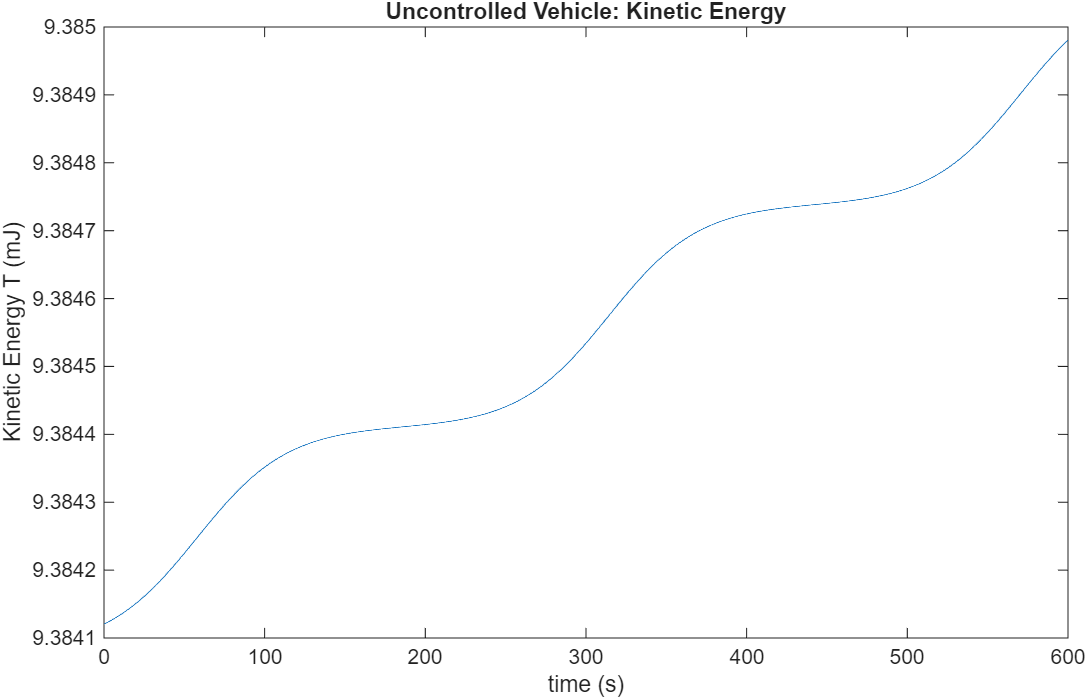
\includegraphics[width=\linewidth]{figures/UncontrolledVehicle_KineticEnergy.png}
			\caption{$\boldsymbol{u}_1$ Applied: $T$}
			\label{fig:u1_T}
		\end{subfigure}
		\hfill
		\begin{subfigure}[b]{0.48\textwidth}
			\centering
			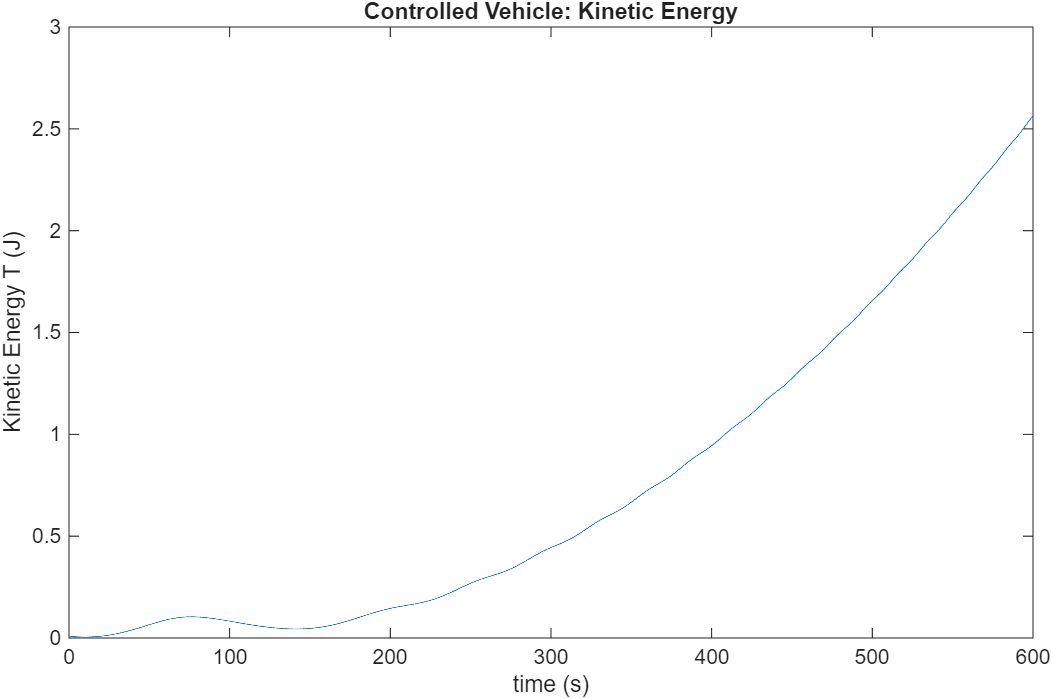
\includegraphics[width=\linewidth]{figures/ControlledVehicle_KineticEnergy.png}
			\caption{$\boldsymbol{u}_2$ Applied: $T$}
			\label{fig:u2_T}
		\end{subfigure}
		
		\vspace{1em} 
		
		\begin{subfigure}[b]{0.48\textwidth}
			\centering
			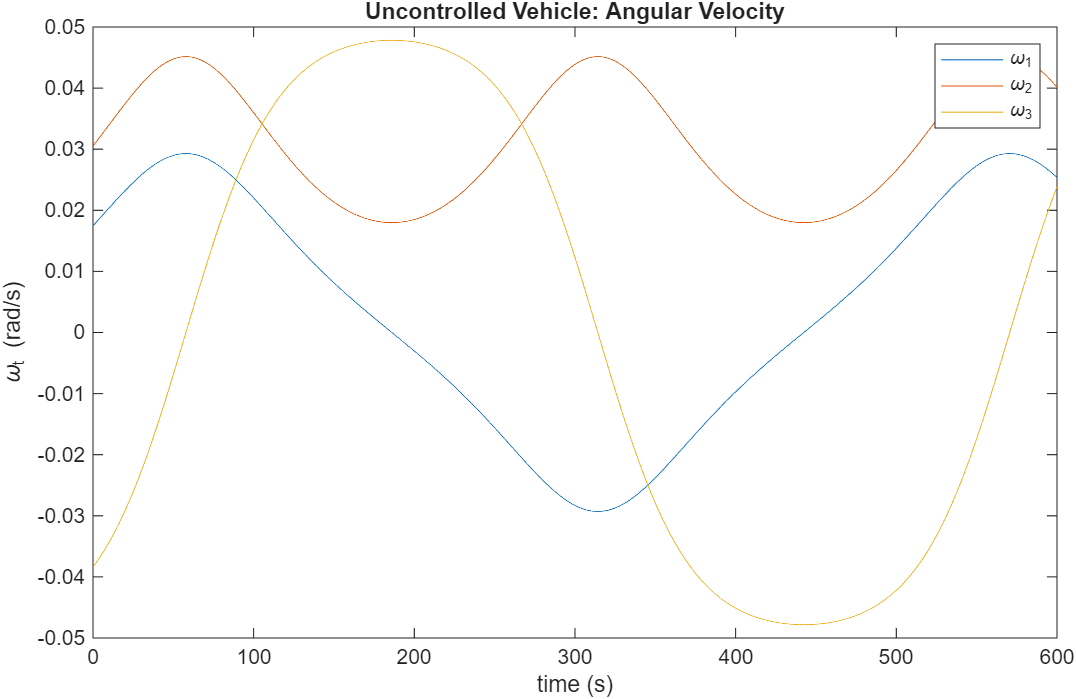
\includegraphics[width=\linewidth]{figures/UncontrolledVehicle_Omega.png}
			\caption{$\boldsymbol{u}_1$ Applied: $\boldsymbol{\omega}_{B/N}$}
			\label{fig:u1_omega}
		\end{subfigure}
		\hfill
		\begin{subfigure}[b]{0.48\textwidth}
			\centering
			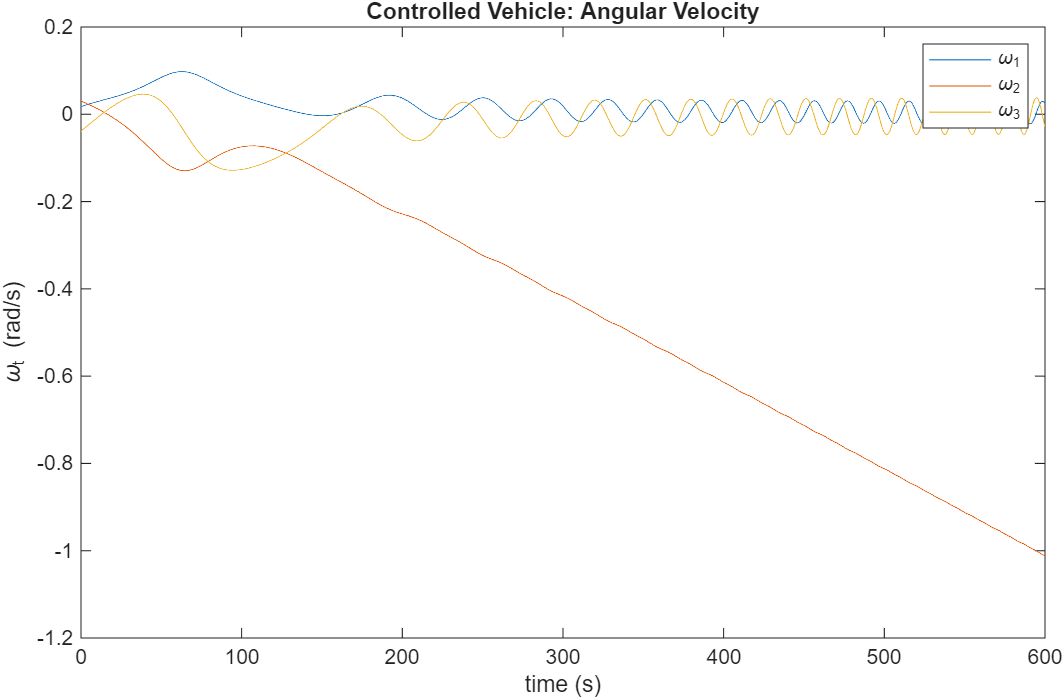
\includegraphics[width=\linewidth]{figures/ControlledVehicle_Omega.png}
			\caption{$\boldsymbol{u}_2$ Applied: $\boldsymbol{\omega}_{B/N}$}
			\label{fig:u2_omega}
		\end{subfigure}
		
		\vspace{1em} 
		
		\begin{subfigure}[b]{0.48\textwidth}
			\centering
			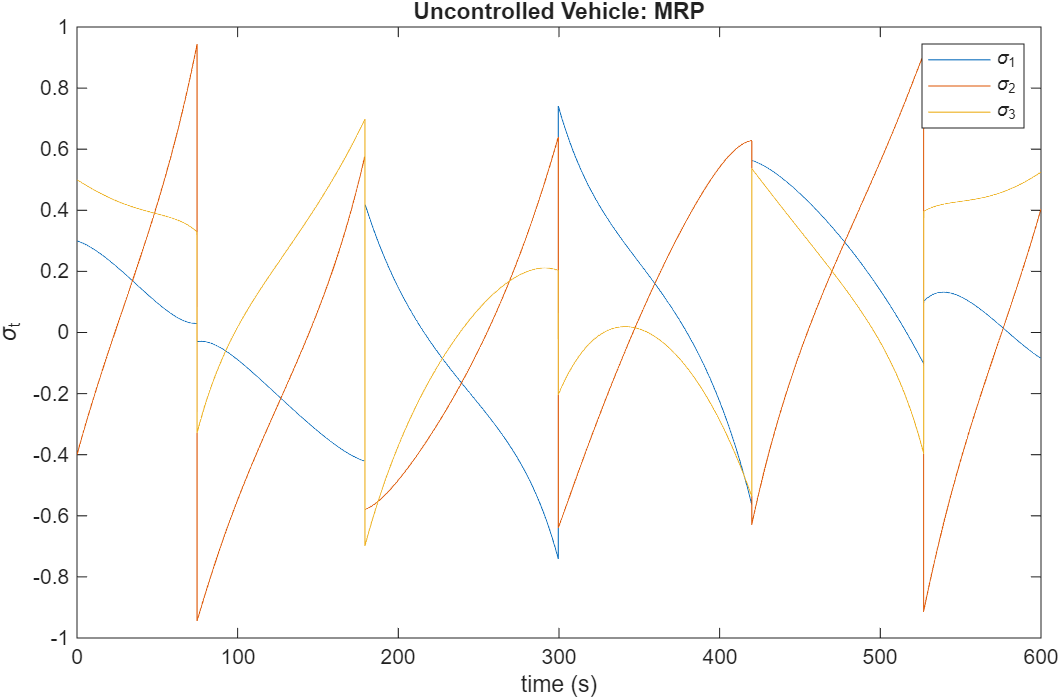
\includegraphics[width=\linewidth]{figures/UncontrolledVehicle_MRP.png}
			\caption{$\boldsymbol{u}_1$ Applied: $\boldsymbol{\sigma}_{B/N}$}
			\label{fig:u1_sigma}
		\end{subfigure}
		\hfill
		\begin{subfigure}[b]{0.48\textwidth}
			\centering
			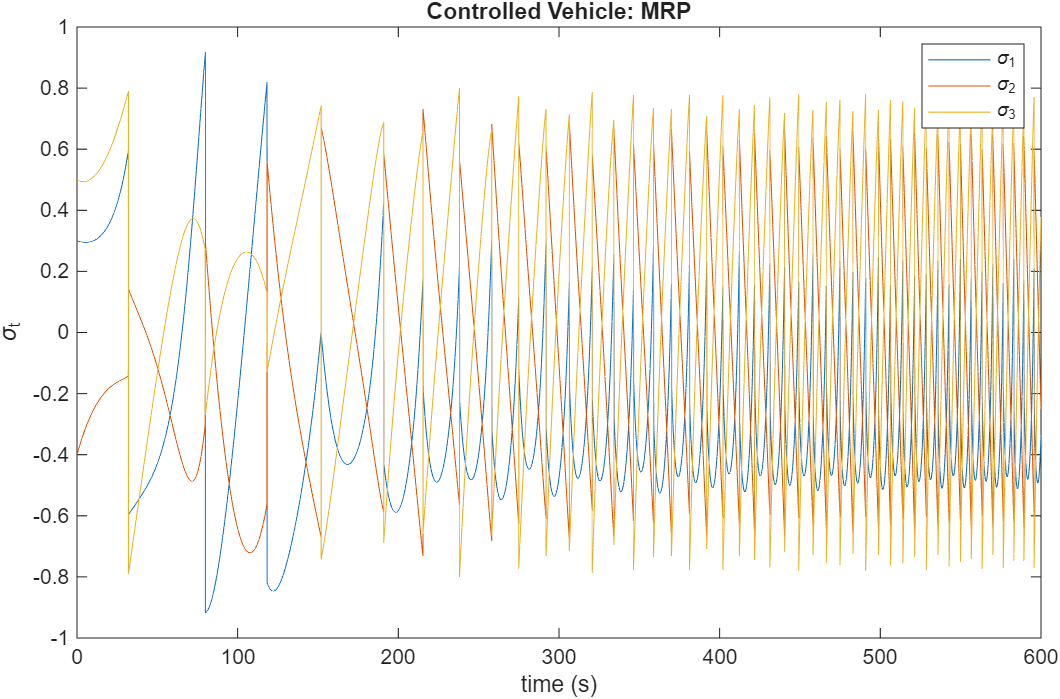
\includegraphics[width=\linewidth]{figures/ControlledVehicle_MRP.png}
			\caption{$\boldsymbol{u}_2$ Applied: $\boldsymbol{\sigma}_{B/N}$}
			\label{fig:u2_sigma}
		\end{subfigure}
		
		
		\caption{Results of the simulations in task 7}
		\label{fig:task7_results}
	\end{figure}
	
	
	\section{Completing the Mission}
	
	\subsection{Task 8: Sun Pointing Control}
	
	The PD gains were selected using the linearized closed-loop attitude dynamics together with a worst-case inertia design approach. Since scalar gains were used for all spacecraft axes, the gains were chosen based on the maximum and minimum principal moments of inertia to guarantee that all rotational modes satisfy the required 120-second decay time constant. 
	
	$$I_{max} = 10, I_{min} = 5$$
	$$T = 120s$$
	
	$$K = \frac{4I_{max}^2}{T^2I_{min}}, P = \frac{2I_{max}}{T}$$
	
	The control torque is defined as:
	
	\[
	\prescript{\mathcal{B}}{}{\boldsymbol{u}} = -K\boldsymbol{\sigma}_{B/R} - P\prescript{\mathcal{B}}{}{\boldsymbol{\omega}}_{B/R}
	\]
	
	An RK4 integrator was developed for pulling off this task used by the MATLAB function \texttt{simulate\_mode()}. The results of Sun pointing simulation are evident in Figure~\ref{fig:sun_pointing}. 
	
	\begin{figure}[H]
		\centering
		
		\begin{subfigure}{0.48\textwidth}
			\centering
			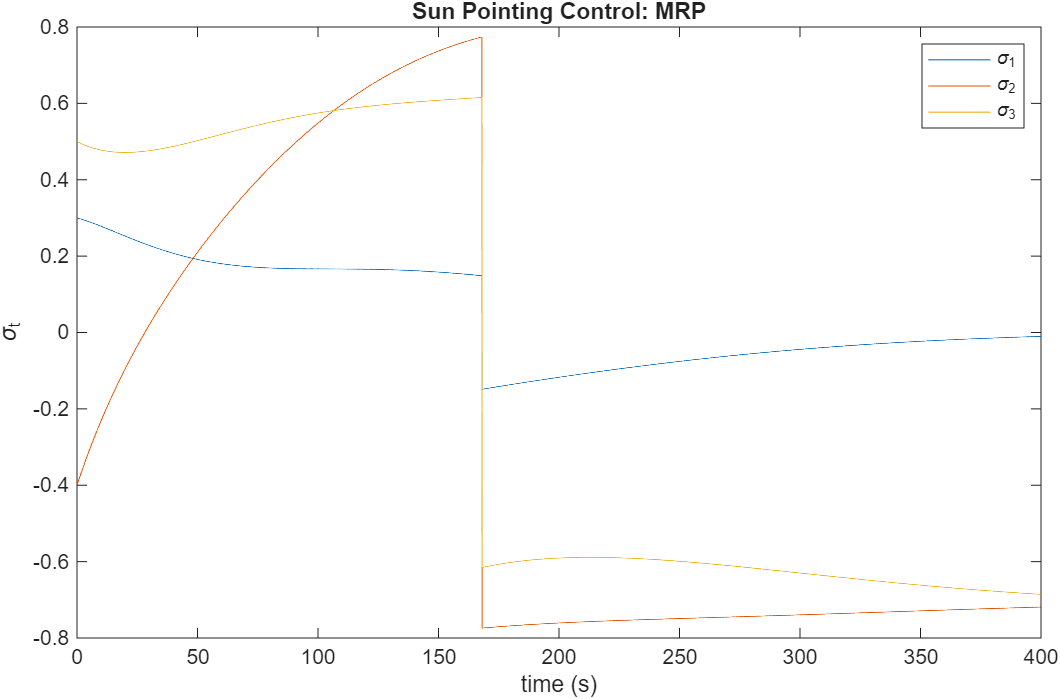
\includegraphics[width=\linewidth]{figures/SunPointing_MRP.png}
			\caption{$\boldsymbol{\sigma}_{B/R}$}
			\label{fig:task8_sigma}
		\end{subfigure}
		\hfill
		\begin{subfigure}{0.48\textwidth}
			\centering
			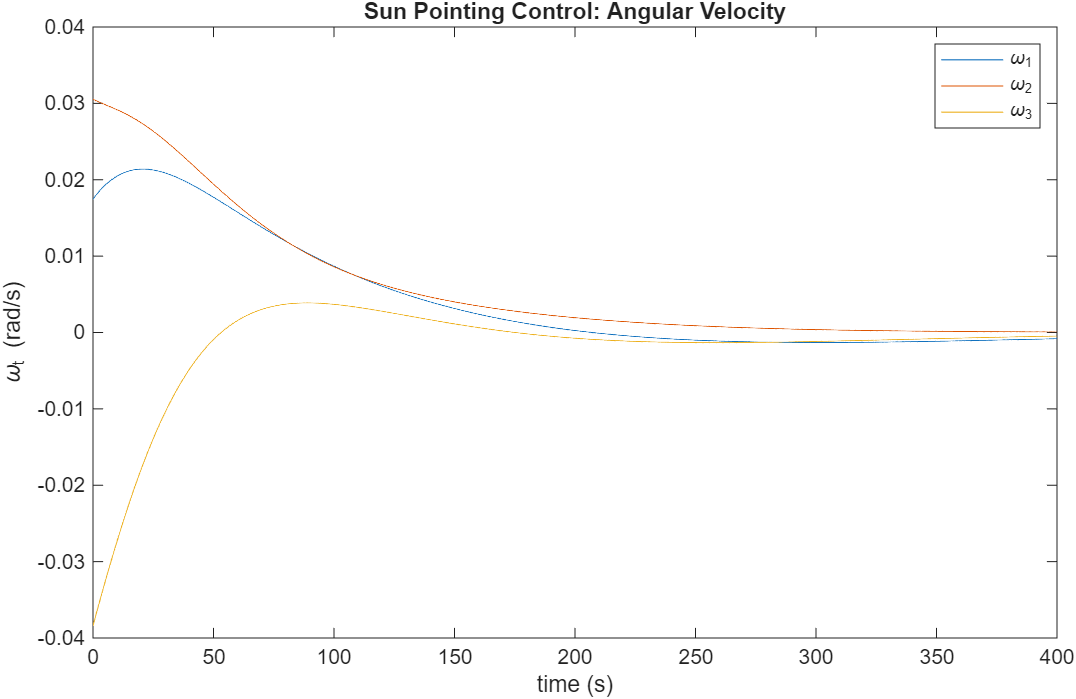
\includegraphics[width=\linewidth]{figures/SunPointing_Omega.png}
			\caption{$\prescript{\mathcal{B}}{}{\boldsymbol{\omega}}_{B/R}$}
			\label{fig:task8_omega}
		\end{subfigure}
		
		\caption{Results of Sun pointing control}
		\label{fig:sun_pointing}
	\end{figure}
	
	As is illustrated, the spacecraft is fully detumbled ($\prescript{\mathcal{B}}{}{\boldsymbol{\omega}}_{B/R} \approx 0$) and controlled to a certain attitude MRP. 
	
	\subsection{Task 9: Nadir Pointing Control}
	
	The same PD control torque developed in task 8 is also applied here and the results of simulation for Nadir pointing mode are evident in Figure~\ref{fig:nadir_pointing}.
	
	\begin{figure}[H]
		\centering
		
		\begin{subfigure}{0.48\textwidth}
			\centering
			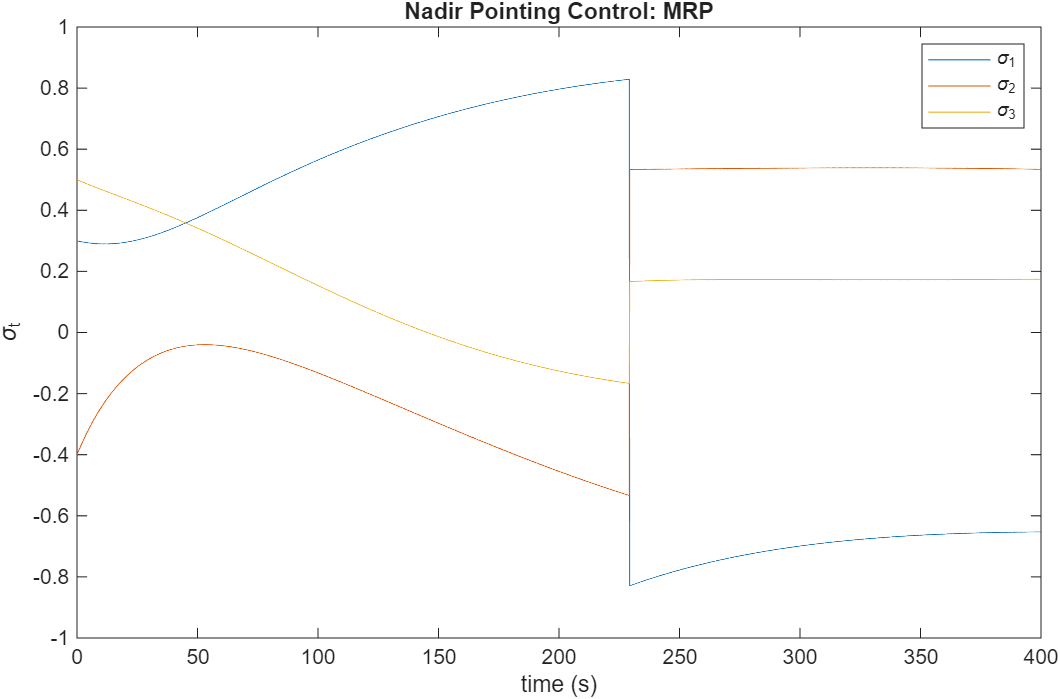
\includegraphics[width=\linewidth]{figures/NadirPointing_MRP.png}
			\caption{$\boldsymbol{\sigma}_{B/R}$}
			\label{fig:task9_sigma}
		\end{subfigure}
		\hfill
		\begin{subfigure}{0.48\textwidth}
			\centering
			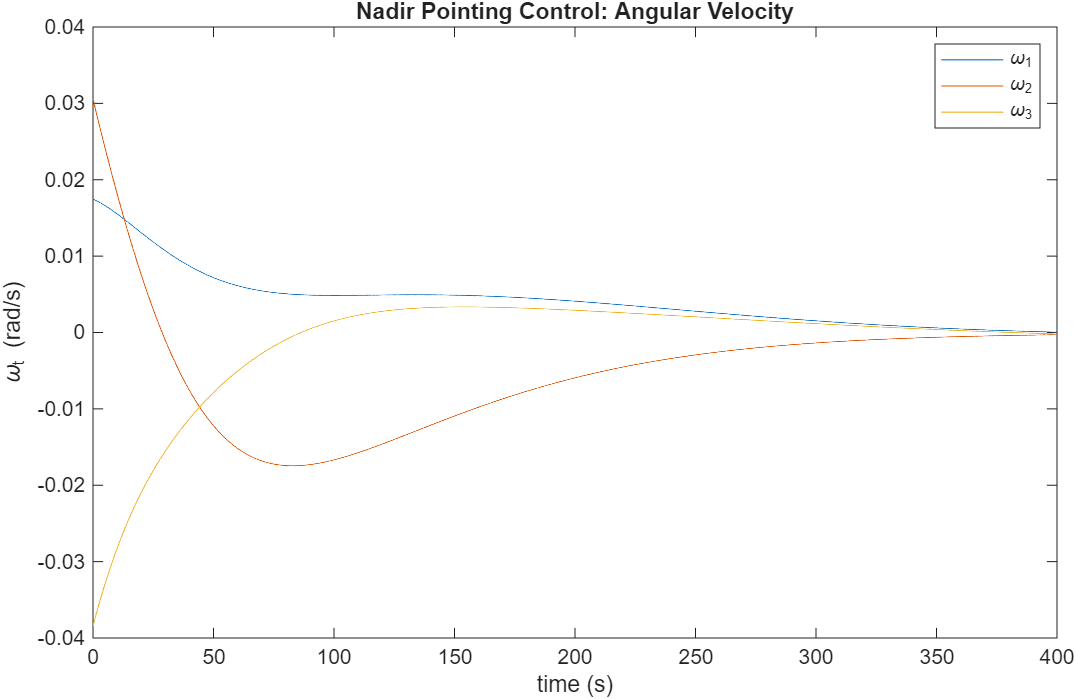
\includegraphics[width=\linewidth]{figures/NadirPointing_Omega.png}
			\caption{$\prescript{\mathcal{B}}{}{\boldsymbol{\omega}}_{B/R}$}
			\label{fig:task9_omega}
		\end{subfigure}
		
		\caption{Results of Nadir pointing control}
		\label{fig:nadir_pointing}
	\end{figure}
	
	Similar to the previous task, the MRP has converged to a certain state and the spacecraft is also detumbled.
	
	\subsection{Task 10: GMO Pointing Control}
	
	The same PD control torque used in two previous tasks is also applied here and the results of simulation for GMO pointing mode are evident in Figure~\ref{fig:GMO_pointing}.
	
	\begin{figure}[H]
		\centering
		
		\begin{subfigure}{0.48\textwidth}
			\centering
			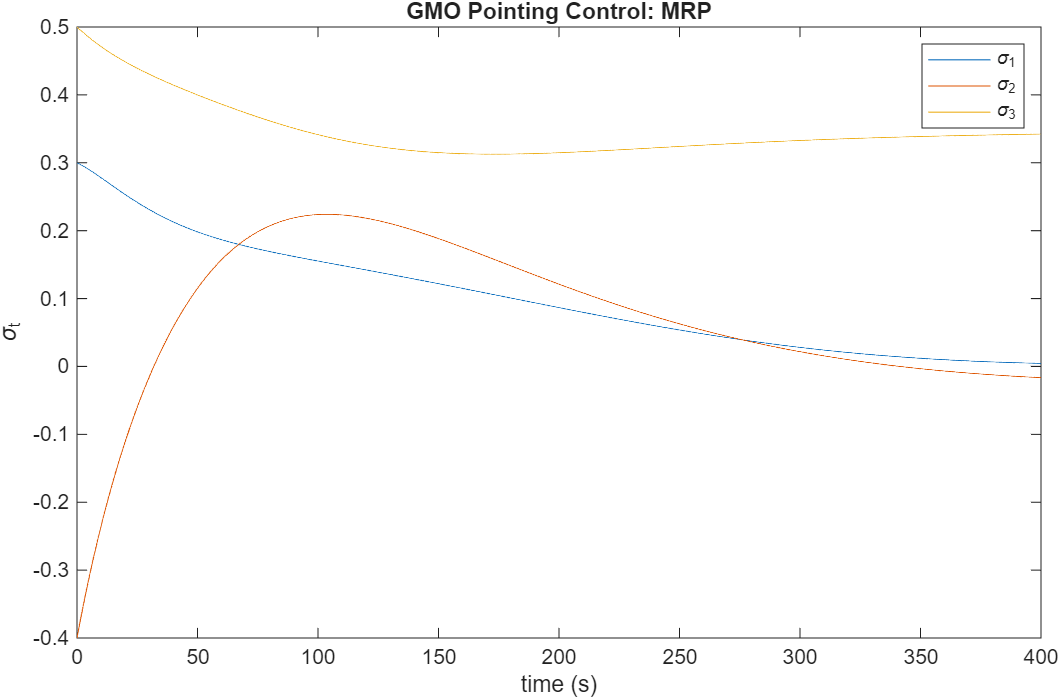
\includegraphics[width=\linewidth]{figures/GMOPointing_MRP.png}
			\caption{$\boldsymbol{\sigma}_{B/R}$}
			\label{fig:task10_sigma}
		\end{subfigure}
		\hfill
		\begin{subfigure}{0.48\textwidth}
			\centering
			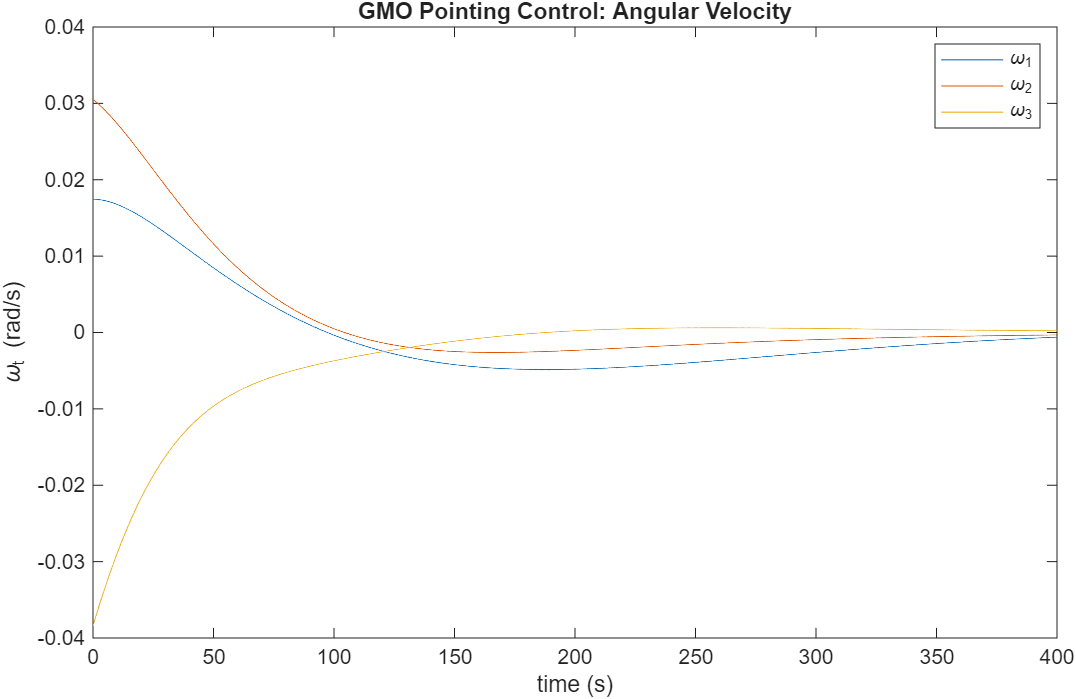
\includegraphics[width=\linewidth]{figures/GMOPointing_Omega.png}
			\caption{$\prescript{\mathcal{B}}{}{\boldsymbol{\omega}}_{B/R}$}
			\label{fig:task10_omega}
		\end{subfigure}
		
		\caption{Results of GMO pointing control}
		\label{fig:GMO_pointing}
	\end{figure}
	
	\subsection{Task 11: Mission Scenario Simulation}
	
	A complete mission simulation was developed to automatically switch between spacecraft operational modes according to mission conditions.
	
	The mission logic was implemented as follows:
	
	\begin{itemize}
		\item If the spacecraft was illuminated by the Sun, Sun-pointing mode was activated,
		\item If the spacecraft was in eclipse and the GMO spacecraft was visible, communication mode was activated,
		\item Otherwise, nadir-pointing science mode was selected.
	\end{itemize}
	
	The task of finding out the operation mode at each given time in the mission--and choosing the corresponding reference frame as a result--is carried out by the MATLAB function \texttt{getReferenceFrame()}. 
	
	
	The MATLAB function \texttt{final\_simulation()} handles the procedure of combining all the modes and tasks together in a timespan of 6500 seconds. 	
	
	\begin{figure}[H]
		\centering
		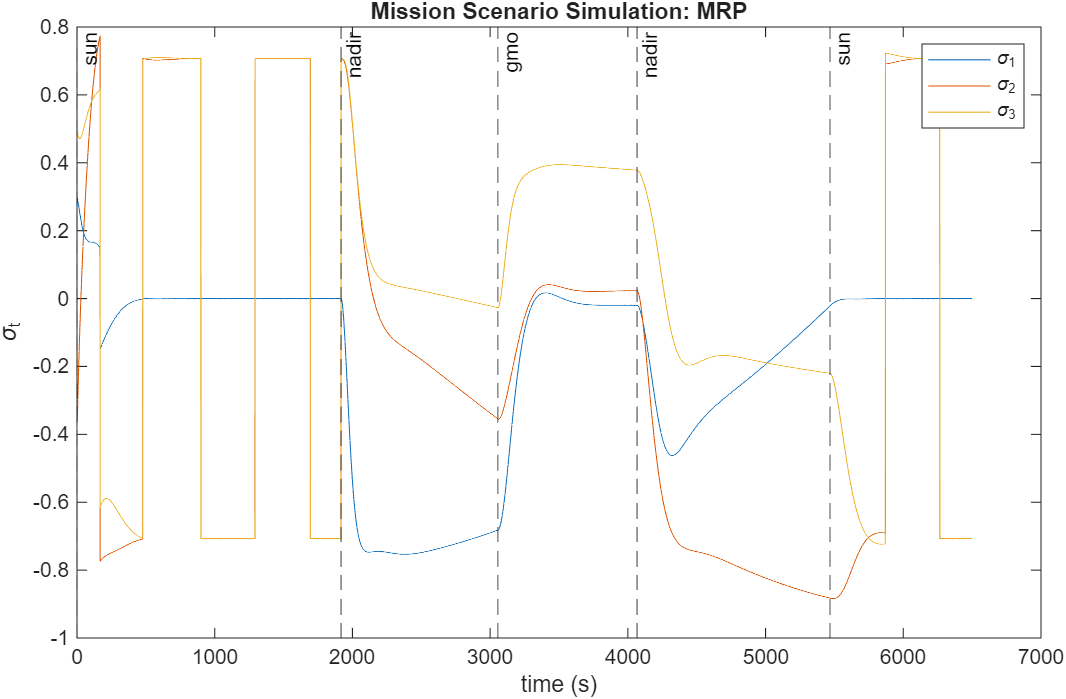
\includegraphics[width=1\textwidth]{figures/mission_sigma.png}
		\caption{Full mission spacecraft attitude state}
		\label{fig:task11_sigma}
	\end{figure}
	
	\begin{figure}[H]
		\centering
		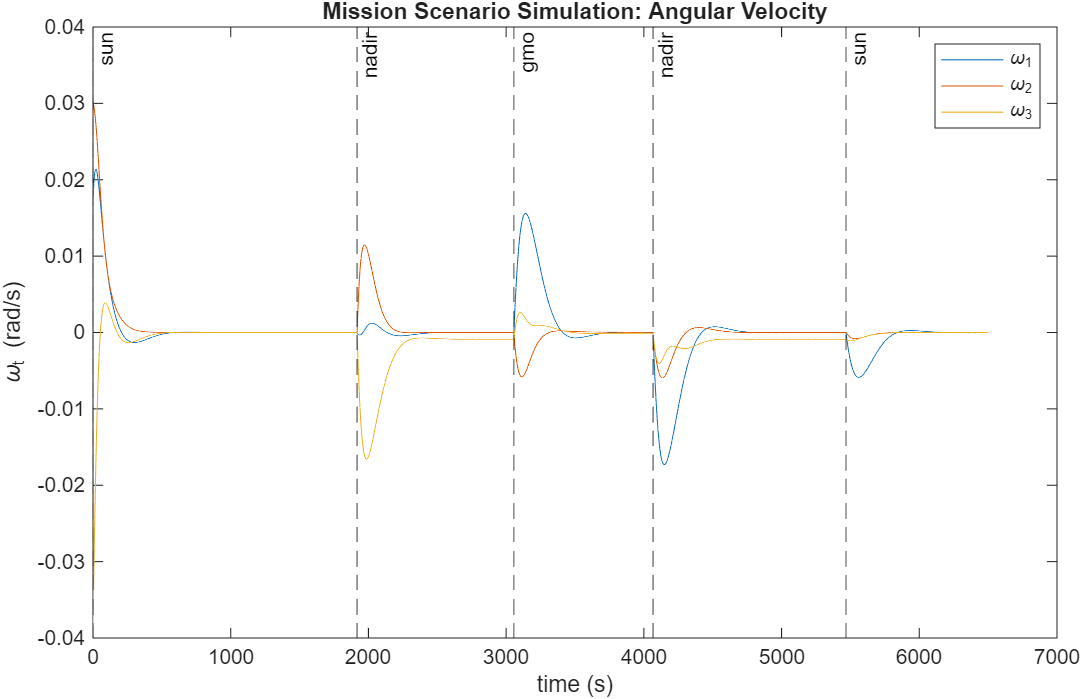
\includegraphics[width=1\textwidth]{figures/mission_omega.png}
		\caption{Full mission spacecraft angular velocity}
		\label{fig:task11_omega}
	\end{figure}
	
	
	\section{Simulation Results and Discussion}
	
	Simulation results demonstrated stable spacecraft attitude behavior under all operational modes. The implemented proportional-derivative controller successfully reduced both attitude and angular velocity tracking errors while maintaining smooth spacecraft rotational motion.
	
	The complete mission simulation validated the autonomous switching architecture between spacecraft operational modes.
	
	\section{STK Visualization}
	
	To validate the MATLAB simulations visually, spacecraft orbit propagation and attitude motion were reconstructed using AGI Systems Tool Kit (STK).
	
	The generated visualization confirmed:
	
	\begin{enumerate}
		\item Correct orbital motion of both spacecraft,
		\item Proper nadir and Sun-pointing orientations,
		\item Communication alignment during GMO visibility windows,
		\item Stable attitude transitions throughout mission operation.
	\end{enumerate}
	
	\section{Appendix: MATLAB Function Overview}
	
	\begin{table}[H]
		\centering
		\caption{Main MATLAB Functions Used in the Project}
		\begin{tabular}{lp{9cm}}
			\toprule
			Function Name & Description \\
			\midrule
			\texttt{orbit\_state()} & Computes spacecraft inertial position and velocity vectors \\
			\texttt{orbitTheta()} & Computes orbital angle evolution \\
			\texttt{orbit\_frame\_dcm()} & Generates Hill-frame DCM \\
			\texttt{RsN\_DCM()} & Returns Sun-pointing reference-frame DCM \\
			\texttt{RnN\_DCM()} & Returns nadir-pointing reference-frame DCM \\
			\texttt{RcN\_DCM()} & Returns GMO-pointing reference-frame DCM \\
			\texttt{attitudeErrorEval()} & Computes tracking errors \\
			\texttt{simulate\_mode()} & Simulates spacecraft attitude dynamics \\
			\texttt{getReferenceFrame()} & Performs automatic mission-mode selection \\
			\bottomrule
		\end{tabular}
	\end{table}
	
	\chapter*{Conclusion}
	\addcontentsline{toc}{chapter}{Conclusion}
	
	This project presented the complete development and implementation of an attitude dynamics and control framework for a nano-satellite orbiting Mars. Multiple mission pointing modes were developed, including Sun-pointing, nadir-pointing, and GMO communication-pointing configurations.
	
	The spacecraft dynamics, reference-frame generation, attitude tracking evaluation, and closed-loop control architecture were successfully implemented in MATLAB and validated through numerical simulation.
	
	The final integrated mission simulation demonstrated stable spacecraft attitude behavior while autonomously switching between operational mission modes according to orbital conditions.
	
	Future improvements may include higher-fidelity environmental disturbance modeling, actuator limitations, sensor-noise modeling, and advanced nonlinear control strategies.
	
\end{document}
